\documentclass[12pt,fleqn]{article}\usepackage{../../common}
\begin{document}
Büyük Sayılar, Veri

Büyük Sayılar Kanunu (Law of Large Numbers)

Bu kanun, örneklem (sample) ile rasgele değişkenler, yani matematiksel
olasılık dağılımları arasında bir bağlantı görevi görür. Kanun kabaca
bildiğimiz günlük bir gerçeğin matematiksel ispatıdır. Yazı-tura atarken
yazı çıkma ihtimalinin 1/2 olduğunu biliyoruz; herhalde çoğumuz bu
yazı-tura işlemin "bir çok kere" tekrarlandığı durumda, toplam sonucun
aşağı yukarı yarısının yazı olacağını bilir.

Matematiksel olarak, farzedelim ki her yazı-tura atışı bir deney
olsun. Deneylerin sonucu $X_1, X_2...X_n$ olarak rasgelen değişkenlerle
olsun, bu değişkenlerin dağılımı aynı (çünkü aynı zar), ve birbirlerinden
bağımsızlar (çünkü her deney diğerinden alakasız). Değişkenlerin sonucu 1
ya da 0 değeri taşıyacak, Yazı=1, Tura=0.

Büyük Sayılar Kanunu tüm bu deney sonuçlarının, yani rasgele değişkenlerin
averajı alınırsa, yani $\bar{X} = X_1 + .. + X_n$ ile, elde edilen sonucun
$X_i$'lerin (aynı olan) beklentisine yaklaşacağının söyler, yani $n$ büyüdükçe
$\bar{X}_n$'in 1/2'ye yaklaştığını ispatlar, yani $E[X_i] = 1/2$
değerine. Notasyonel olarak $E(X_i) = \mu$ olarak da gösterilebilir.

Özetlemek gerekirse, bir olasılık dağılımına sahip olan, görmediğimiz bir
``yerlerde'' olan bir dağılımdan bir örneklem alıyoruz, örneklem bir zar
atma işlemi gibi (simülasyon ile bu değişkenleri de doldurabilirdik), sonra
bu değişkenlerin averajını alıyoruz, ve bu averajın o görmediğimiz
bilmediğimiz ``gerçek'' dağılımın $\mu$ değerine yaklaştığını görüyoruz. 

Formülsel olarak, herhangi bir $\epsilon > 0$ için,

$$ \lim_{n \to \infty} P(|\bar{X} - \mu| \le \epsilon) = 1$$

ya da

 $$ \lim_{n \to \infty} P(|\bar{X}_n-\mu| > \epsilon) = 0 $$

ya da 

$$ P(|\bar{X}_n-\mu| > \epsilon) \rightarrow 0 $$

Burada ne söylendiğine dikkat edelim, $X_i$ dağılımı {\em ne olursa olsun}, yanı
ister Binom, ister Gaussian olsun, {\em örneklem} üzerinden hesaplanan sayısal
ortalamanın (empirical mean) formülsel olasılık beklentisine yaklaştığını
söylüyoruz! $X_i$'ler en absürt dağılımlar olabilirler, bu dağılımların
fonksiyonu son derece çetrefil, tek tepeli (unimodal) bile olmayabilir, o
formüller üzerinden beklenti için gereken entegralin belki analitik çözümü bile
mevcut olmayabilir! Ama yine de ortalama, o dağılımların beklentisine
yaklaşacaktır.  İstatistik ile olasılık teorisi arasındaki çok önemli bir
bağlantı bu.

Sonuç şaşırtıcı, fakat bir ek daha yapalım, sezgisel (intuitive) olarak
bakarsak aslında sonuç çok şaşırtıcı olmayabilir. Niye? Diyelim ki genel
veri $N(\mu,\sigma^2)$ şeklinde bir Normal dağılımdan geliyor ve örneklem
de bu sebeple aynı dağılıma sahip. Bu durumda örneklemdeki veri
noktalarının $\mu$'ya yakın değerler olmasını beklemek mantıklı olmaz mı?
Çünkü bu dağılım ``zar atınca'' ya da bir genel nüfustan bir ``örnek
toplayınca'' (ki bunu bir anlamda istatistiksel bir zar atışı olarak
görebiliriz) onu $\mu,\sigma^2$'e göre atacak. Örneklemi zar atışı
sonuçları olarak gördüğümüze göre elde edilen verilerin bu şekilde olacağı
şaşırtıcı olmamalı. Ve bu zar atışlarının ortalamasının, son derece basit
bir aritmetik bir işlemle hesaplanıyor olsa bile, $\mu$'ye yaklaşması
normal olmalı.

Bu arada, bu argümana tersten bakarsak Monte Carlo entegralinin niye
işlediğini görebiliriz, bkz [3].

Özellikle örneklem ile genel nüfus (population) arasında kurulan bağlantıya
dikkat edelim. İstatiğin önemli bir bölümünün bu bağlantı olduğu
söylenebilir. Her örneklem, bilmediğimiz ama genel nüfusu temsil eden bir
dağılımla aynı dağılıma sahip olan $X_i$'dir dedik, ve bu aynılıktan ve
bağımsızlıktan yola çıkarak bize genel nüfus hakkında bir ipucu sağlayan
bir kanun geliştirdik (ve birazdan ispatlayacağız).

İspata başlayalım.

$X_1,X_2,..,X_n$ bağımsız değişkenler olsun. 

$$ E(X_i) = \mu $$

$$ Var(X_i) = \sigma $$

$$ \bar{X}_n = \frac{1}{n} \sum_{i=1}^n X_i  $$

$\bar{X}_n$ de bir rasgele değişkendir, çünku $\bar{X}_n$ değişkeni her
$X_i$ dağılımıyla alakalı.

İspata devam etmek için $\bar{X}_n$ dağılımının beklentisini bulmamız gerekiyor.

$$ E(\bar{X}_n) = E(\frac{1}{n} \sum_{i=1}^n X_i)  $$

E doğrusal bir işleç (linear operatör) olduğu için dışarıdan içeri doğru
nüfuz eder. 

$$ = \frac{1}{n} \sum_{i=1}^n E(X_i) = \frac{1}{n}n\mu = \mu $$

Dikkat edelim, bu {\em ortalamanın} beklentisi, ortalamanın kendisinin
hangi değere yaklaşacağını hala göstermiyor. Eğer öyle olsaydı işimiz
bitmiş olurdu :) Daha yapacak çok iş var.

Şimdi $\bar{X}_n$ dağılımının standart sapmasını da bulalım. Diğer bir
olasılık kuramına göre

$$ Y = a + bX $$

$$ Var(Y) = b^2Var(X) $$

oldugunu biliyoruz. O zaman,

$$ \bar{X}_n = \frac{1}{n} \sum_{i=1}^n X_i  $$

$$ Var(\bar{X}_n) = Var(\frac{1}{n}\sum_{i=1}^nX_i) = 
\frac{1}{n^2}\sum_{i=1}^n Var(X_i)
$$

$$ 
Var(\bar{X}_n) = \frac{1}{n^2}\sum_{i=1}^n \sigma^2 = 
\frac{1}{n^2}n\sigma^2 = \frac{\sigma^2}{n} 
\mlabel{3}
$$

Artık Çebişev kuramını kullanmaya hazırız. Ispatlamaya calistigimiz neydi?
$n \rightarrow \infty$ iken,

 $$ P(|\bar{X}_n-\mu| > \epsilon) \rightarrow 0 $$

Çebişev'den

$$ P(|\bar{X}_n-\mu| > \epsilon) \le \frac{Var(\bar{X}_n)}{\epsilon^2} $$

$$ P(|\bar{X}_n-\mu| > \epsilon) \le \frac{\sigma^2}{n\epsilon^2}
\rightarrow 0 $$

$\sigma^2 / n\epsilon^2$'in sıfıra gitmesi normal çünkü $n$ sonsuza gidiyor.

Peki $P(|\bar{X}_n-\mu| > \epsilon)$'nin sıfıra gittiğini gösterdik mi? 

$\sigma^2 / n\epsilon^2$'nin sıfıra gittiğini gösterdik. $\sigma^2 /
n\epsilon^2$ de $P(|\bar{X}_n-\mu| > \epsilon)$'den büyük olduğuna göre, demek
ki o da sıfıra iner.

Çebişev Eşitsizliğinin ispatı ek bölümde bulunabilir.

$\square$

Büyük Sayılar Kanunu örneklem ortalamasının ve varyansının $X_i$'in
beklentisi ve varyansı ile bağlantı kurar. Merkezi Limit Teorisi bir adım
daha atar, ve der ki ``$\bar{X}$'in dağılımı Gaussian dağılım olmalıdır
yani normal eğrisi şeklinde çıkmalıdır!''. Teorinin detayları bu bölümde
bulunabilir. 

Merkezi Limit Teorisi (Central Limit Theorem -CLT-)

Büyük Sayılar Kanunu örneklem ortalamasının gerçek nüfus beklentisine
yaklaşacağını ispatladı. Örneklem herhangi bir dağılımdan
gelebiliyordu. CLT bu teoriyi bir adım ilerletiyor ve diyor ki kendisi de
bir rasgele değişken olan örneklem ortalaması $\bar{X}$ Normal dağılıma
sahiptir! Daha detaylandırmal gerekirse, 

Diyelim ki $X_1,..,X_i$ örneklemi birbirinden bağımsız, aynı dağılımlı ve
ortalaması $\mu$, standart sapması $\sigma$ olan (ki o da aynı dağılıma
sahip) bir nüfustan geliyorlar. Örneklem ortalaması $\bar{X}$, ki bu
rasgele değişkenin beklentisinin $\mu$, ve (3)'e göre standart sapmasının
$\sigma / \sqrt{n}$ olduğunu biliyoruz. Dikkat: $\bar{X}$'in kendisinden
değil, {\em beklentisinden} bahsediyoruz, BSK'deki aynı durum, yani
ortalama dağılımının ortalaması. Teori der ki $n$ büyüdükçe $\bar{X}$
dağılımı (bu sefer kendisi) bir $N(\mu, \sigma/\sqrt{n})$ dağılımına
yaklaşır.

Bu ifade genelde standart normal olarak gösterilir, herhangi bir normal
dağılımı standart normal'e dönüştürmeyi daha önce görmüştük zaten,
beklentiyi çıkartıp standart sapmaya bölüyoruz, o zaman örneklem dağılımı
$\bar{X}$,

$$ Z = \frac{\bar{X} - \mu}{\sigma / \sqrt{n}} $$

dağılımına yaklaşır diyoruz, ki $Z = N(0,1)$ dağılımıdır, beklentisi sıfır,
standart sapması 1 değerindedir. 

Bu teorinin ispatını şimdilik vermeyeceğiz. 

Parametre Tahmin Ediciler (Estimators) 

Maksimum Olurluk (maximum likelihood) kavramını kullanarak ilginç bazı
sonuçlara erişmek mümkün; bu sayede dağılım fonksiyonları ve veri arasında
bazı sonuçlar elde edebiliriz. Maksimum olurluk nedir? MO ile verinin her
noktası teker teker olasılık fonksiyonuna geçilir, ve elde edilen olasılık
sonuçları birbiri ile çarpılır. Çoğunlukla formül içinde bilinmeyen
bir(kaç) parametre vardır, ve bu çarpım sonrası, içinde bu parametre(ler)
olan yeni bir formül ortaya çıkar. Bu nihai formülün kısmi türevi alınıp
sıfıra eşitlenince cebirsel bazı teknikler ile bilinmeyen parametre
bulunabilir. Bu sonuç eldeki veri bağlamında en mümkün (olur) parametre
değeridir. Öyle ya, mesela Gaussian $N(10,2)$ dağılımı var ise, 60,90 gibi
değerlerin ``olurluğu'' düşüktür. Gaussin üzerinde örnek,

$$
f(x;\mu,\sigma) = \frac{1}{\sigma\sqrt{2\pi}} 
\exp \bigg\{ - \frac{1}{2\sigma^2}(x-\mu)^2  \bigg\}
, \ x \in \mathbb{R}
$$
 
Çarpım sonrası

$$ f(x_1,..,x_n;\mu,\sigma) = 
\prod \frac{1}{\sigma\sqrt{2\pi}} 
\exp \bigg\{ - \frac{1}{2\sigma^2}(x_i-\mu)^2  \bigg\}
$$

$$ =
\frac{(2\pi)^{-n/2}}{\sigma^n}
\exp \bigg\{ - \frac{\sum (x_i-\mu)^2}{2\sigma^2}  \bigg\}
$$

Üstel kısım $-n/2$ nereden geldi? Çünkü bölen olan karekökü üste çıkardık,
böylece $-1/2$ oldu, $n$ çünkü $n$ tane veri noktası yüzünden formül $n$
kere çarpılıyor. Veri noktaları $x_i$ içinde. Eğer log, yani $\ln$ alırsak
$\exp$'den kurtuluruz, ve biliyoruz ki log olurluğu maksimize etmek normal
olurluğu maksimize etmek ile aynı şeydir, çünkü $\ln$ transformasyonu
monoton bir transformasyondur. Ayrıca olurluk içbukeydir (concave) yani
kesin tek bir maksimumu vardır. 

$$ \ln f = -\frac{1}{2} n \ln (2\pi) 
- n \ln \sigma - 
\frac{\sum (x_i-\mu)^2}{2\sigma^2}  
$$

Türevi alıp sıfıra eşitleyelim

$$ \frac{\partial (\ln f)}{\partial \mu} =
\frac{\sum (x_i-\mu)^2}{2\sigma^2}   = 0 
$$

$$ \hat{\mu} = \frac{\sum x_i }{n} $$

Bu sonuç (1)'deki formül, yani örneklem ortalaması ile aynı! Fakat buradan
hemen bir bağlantıya zıplamadan önce şunu hatırlayalım - örneklem
ortalaması formülünü {\em biz} tanımladık. ``Tanım'' diyerek bir ifade
yazdık, ve budur dedik. Şimdi sonradan, verinin dağılımının Gaussian
olduğunu farzederek, bu verinin mümkün kılabileceği en optimal parametre
değeri nedir diye hesap ederek aynı formüle eriştik, fakat bu bir anlamda
bir güzel raslantı oldu.. Daha doğrusu bu aynılık Gaussian / Normal
dağılımlarının ``normalliği'' ile alakalı muhakkak, fakat örnekleme
ortalaması hiçbir dağılım faraziyesi yapmıyor, herhangi bir dağılımdan
geldiği bilinen ya da bilinmeyen bir veri üzerinde kullanılabiliyor. Bunu
unutmayalım. İstatistikte matematiğin lakaytlaşması (sloppy) kolaydır, o
sebeple neyin tanım, neyin hangi faraziyeye göre optimal, neyin nüfus
(population) neyin örneklem (sample) olduğunu hep hatırlamamız lazım.

Devam edelim, maksimum olurluk ile $\hat{\sigma}$ hesaplayalım,

$$ \frac{\partial (\ln f)}{\partial \sigma} =
-\frac{n}{\sigma} + \frac{\sum (x_i-\mu)^2}{2\sigma^3}   = 0 
$$

Cebirsel birkac duzenleme sonrasi ve $\mu$ yerine yeni hesapladigimiz
$\hat{\mu}$ kullanarak,

$$ \hat{\sigma}^2 = \frac{\sum (x_i-\hat{\mu})^2}{n} $$

Bu da örneklem varyansı ile aynı! 

Yansızlık (Unbiasedness)

Tahmin edicilerin kendileri de birer rasgele değişken olduğu için her
örneklem için değişik değerler verirler. Diyelim ki $\theta$ için bir
tahmin edici $\hat{\theta}$ hesaplıyoruz, bu $\hat{\theta}$ gerçek $\theta$
için bazı örneklemler için çok küçük, bazı örneklemler için çok büyük
sonuçlar (tahminler) verebilecektir. Kabaca ideal durumun, az çıkan
tahminlerin çok çıkan tahminleri bir şekilde dengelemesi olduğunu tahmin
edebiliriz, yani tahmin edicinin üreteceği pek çok değerin $\theta$'yı bir
şekilde ``ortalaması'' iyi olacaktır.

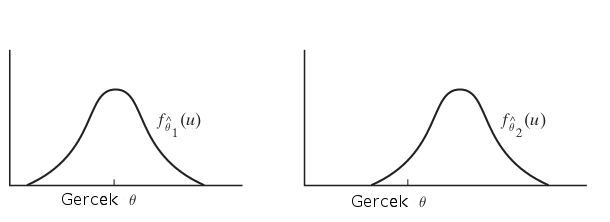
\includegraphics[height=5cm]{unbias.png}

Bu durumu şöyle açıklayalım, madem tahmin ediciler birer rasgele değişken,
o zaman bir dağılım fonksiyonları var. Ve üstteki resimde örnek olarak
$\hat{\theta_1},\hat{\theta_2}$ olarak iki tahmin edici gösteriliyor mesela
ve onlara tekabül eden yoğunluklar $f_{\hat{\theta_1}},
f_{\hat{\theta_1}}$. İdeal durum soldaki resimdir, yoğunluğun fazla olduğu
yer gerçek $\theta$'ya yakın olması. Bu durumu matematiksel olarak nasıl
belirtiriz? Beklenti ile!

Tanım

$Y_1,..,Y_n$ üzerindeki $\theta$ tahmin edicisi $\hat{\theta} $'den alınmış
rasgele örneklem. Eğer tüm $\theta$'lar için $E(\hat{\theta}) = \theta$
işe, bu durumda tahmin edicinin yansız olduğu söylenir.

Örnek olarak maksimum olurluk ile önceden hesapladığımız $\hat{\sigma}$
tahmin edicisine bakalım. Bu ifade

$$ \hat{\sigma}^2 = \frac{1}{n}\sum (Y_i-\hat{\mu})^2 $$

ya da 

$$ \hat{\sigma}^2 = \frac{1}{n}\sum_i (Y_i-\bar{Y})^2 $$

ile belirtildi. Tahmin edici $\hat{\sigma}^2$, $\sigma^2$ için yansız midir?
Tanımımıza göre eğer tahmin edici yansız ise $E(\hat{\sigma}^2) = \sigma^2$
olmalıdır.

Not: Faydalı olacak bazı eşitlikler, daha önceden gördüğümüz

$$ Var(X) = E(X^2) - (E(X)^2)$$

ve sayısal ortalama $\bar{Y}$'nin beklentisi $E({\bar{Y}}) = E(Y_i)$, ve
$Var(\bar{Y}) = 1/n Var(Y_i)$.

Başlayalım,

$$ E(\hat{\sigma}^2) = E\bigg(\frac{1}{n}\sum_i (Y_i-\bar{Y})^2 \bigg)$$

Parantez içindeki $1/n$ sonrasındaki ifadeyi açarsak,


$$ \sum_i (Y_i-\bar{Y})^2  =  \sum_i (Y_i^2-2Y_i\bar{Y}+ \bar{Y}^2)$$

$$ = \sum_iY_i^2 -2\sum_i Y_i\bar{Y} + n\bar{Y}^2  $$

$\sum_i Y_i$'nin hemen yanında $\bar{Y}$ görüyoruz. Fakat $\bar{Y}$'nin kendisi
zaten $1/n \sum_i Y_i$ demek değil midir? Ya da, toplam içinde her $i$ için
değişmeyecek $\bar{Y}$'yi toplam dışına çekersek, $\bar{Y}\sum_iY_i$ olur, bu da
$\bar{Y} \cdot n \bar{Y}$ demektir ya da $n\bar{Y}^2$,

$$ = \sum_iY_i^2 -2 n\bar{Y}^2 + n\bar{Y}^2  $$

$$ = \sum_iY_i^2 -n\bar{Y}^2  $$

Dikkat, artık $-n\bar{Y}^2$ toplama işleminin {\em dışında}. Şimdi beklentiye
geri dönelim,

$$ = E \bigg( \frac{1}{n} \bigg( \sum_iY_i^2 -n\bar{Y}^2 \bigg) \bigg) $$

$1/n$ dışarı çekilir, beklenti toplamdan içeri nüfuz eder,

$$ = \frac{1}{n} \bigg(  \sum_i  E(Y_i^2) -n E(\bar{Y}^2) \bigg) $$

Daha önce demiştik ki (genel bağlamda)

$$ Var(X) = E(X^2) - (E(X)^2)$$

Bu örnek için harfleri değiştirirsek,

$$ Var(Y_i) = E(Y_i^2) - E(Y_i)^2$$

Yani

$$ E(Y_i^2) = Var(Y_i) + E(Y_i)^2 $$

$E(Y_i) = \mu$ oldugunu biliyoruz,

$$ E(Y_i^2) = Var(Y_i) + \mu^2 $$

Aynısını $ E(\bar{Y}^2)$ için kullanırsak,

$$  E(\bar{Y}^2) = Var(\bar{Y}) + E(\bar{Y})^2 $$

$E(\bar{Y}) = \mu$, 

$$  E(\bar{Y}^2) = Var(\bar{Y}) + \mu^2 $$

$$
= \frac{1}{n} \bigg(  \sum_i Var(Y_i) + \mu^2   
-n (Var(\bar{Y}) + \mu^2 ) \bigg) 
$$

$Var(Y_i) = \sigma$, ve başta verdiğimiz eşitlikler ile beraber

$$
= \frac{1}{n} \bigg(  \sum_i (\sigma^2 + \mu^2)
-n (\frac{\sigma^2}{n} + \mu^2 ) \bigg) 
$$

Tekrar hatırlatalım, $\sum_i$ sadece ilk iki terim için geçerli, o zaman,
ve sabit değerleri $n$ kadar topladığımıza göre bu aslında bir çarpım
işlemi olur,

$$ 
= \frac{1}{n} \bigg(  n\sigma^2 + n\mu^2   
-n (\frac{\sigma^2}{n} + \mu^2 ) \bigg) 
$$

$$ 
=  \sigma^2 + \mu^2 -\frac{\sigma^2}{n} - \mu^2 
$$

$$ 
=  \sigma^2 -\frac{\sigma^2}{n} 
$$

$$ 
=  \frac{n\sigma^2}{n} -\frac{\sigma^2}{n} 
$$


$$ 
=  \frac{n\sigma^2 - \sigma^2}{n} 
$$

$$ 
=  \frac{\sigma^2(n-1)}{n} 
$$

$$ = \sigma^2 \frac{n-1}{n} $$

Görüldüğü gibi eriştiğimiz sonuç $\sigma^2$ değil, demek ki bu tahmin edici
yansız değil. Kontrol tamamlandı.

Fakat eriştiğimiz son denklem bize başka bir şey gösteriyor, eğer üstteki
sonucu $\frac{n}{n-1}$ ile çarpsaydık, $\sigma^2$ elde etmez miydik? O
zaman yanlı tahmin ediciyi yansız hale çevirmek için, onu $\frac{n}{n-1}$
ile çarparız ve

$$ \frac{n}{n-1} \frac{1}{n}\sum_i (Y_i-\bar{Y})^2 $$

$$ =  \frac{1}{n-1}\sum_i (Y_i-\bar{Y})^2 $$

Üstteki ifade $\sigma^2$'nin yansız tahmin edicisidir. 

Hesap için kullandığınız kütüphanelerin yanlı mı yansız mı hesap yaptığını
bilmek iyi olur, mesela Numpy versiyon 1.7.1 itibariyle yanlı standart
sapma hesabı yapıyor, fakat Pandas yansız olanı kullanıyor (Pandas
versiyonu daha iyi)

\begin{minted}[fontsize=\footnotesize]{python}
import pandas as pd
arr = np.array([1,2,3])
print 'numpy', np.std(arr)
print 'pandas', float(pd.DataFrame(arr).std())
\end{minted}

\begin{verbatim}
numpy 0.816496580928
pandas 1.0
\end{verbatim}

Kaynaklar

[1] Wolfram Mathworld, {\em Maximum Likelihood}, \url{http://mathworld.wolfram.com/MaximumLikelihood.html}

[2] {\em Introduction to Probability and Statistics Using R}

[3] Bayramlı, Istatistik, {\em Monte Carlo, Entegraller, MCMC}



\end{document}


